%% Version 4.3.2, 25 August 2014
%
%%%%%%%%%%%%%%%%%%%%%%%%%%%%%%%%%%%%%%%%%%%%%%%%%%%%%%%%%%%%%%%%%%%%%%
% Template.tex --  LaTeX-based template for submissions to the 
% American Meteorological Society
%
% Template developed by Amy Hendrickson, 2013, TeXnology Inc., 
% amyh@texnology.com, http://www.texnology.com
% following earlier work by Brian Papa, American Meteorological Society
%
% Email questions to latex@ametsoc.org.
%
%%%%%%%%%%%%%%%%%%%%%%%%%%%%%%%%%%%%%%%%%%%%%%%%%%%%%%%%%%%%%%%%%%%%%
% PREAMBLE
%%%%%%%%%%%%%%%%%%%%%%%%%%%%%%%%%%%%%%%%%%%%%%%%%%%%%%%%%%%%%%%%%%%%%

%% Start with one of the following:
% DOUBLE-SPACED VERSION FOR SUBMISSION TO THE AMS
%\documentclass{ametsoc}

% TWO-COLUMN JOURNAL PAGE LAYOUT---FOR AUTHOR USE ONLY
\documentclass[twocol]{ametsoc}
\usepackage{arydshln}

%%%%%%%%%%%%%%%%%%%%%%%%%%%%%%%%
%%% To be entered only if twocol option is used

\journal{jamc}

%  Please choose a journal abbreviation to use above from the following list:
% 
%   jamc     (Journal of Applied Meteorology and Climatology)
%   jtech     (Journal of Atmospheric and Oceanic Technology)
%   jhm      (Journal of Hydrometeorology)
%   jpo     (Journal of Physical Oceanography)
%   jas      (Journal of Atmospheric Sciences)	
%   jcli      (Journal of Climate)
%   mwr      (Monthly Weather Review)
%   wcas      (Weather, Climate, and Society)
%   waf       (Weather and Forecasting)
%   bams (Bulletin of the American Meteorological Society)
%   ei    (Earth Interactions)

%%%%%%%%%%%%%%%%%%%%%%%%%%%%%%%%
%Citations should be of the form ``author year''  not ``author, year''
%\bibpunct{(}{)}{;}{a}{}{,}

%%%%%%%%%%%%%%%%%%%%%%%%%%%%%%%%

%%% To be entered by author:

%% May use \\ to break lines in title:

\title{Metadata Load Balancing Policies and Key-Value Stores}

%%% Enter authors' names, as you see in this example:
%%% Use \correspondingauthor{} and \thanks{Current Affiliation:...}
%%% immediately following the appropriate author.
%%%
%%% Note that the \correspondingauthor{} command is NECESSARY.
%%% The \thanks{} commands are OPTIONAL.

    %\authors{Author One\correspondingauthor{Author One, 
    % American Meteorological Society, 
    % 45 Beacon St., Boston, MA 02108.}
% and Author Two\thanks{Current affiliation: American Meteorological Society, 
    % 45 Beacon St., Boston, MA 02108.}}

\authors{Michael Sevilla\correspondingauthor{Los Alamos National Laboratory}}

%% Follow this form:
    % \affiliation{American Meteorological Society, 
    % Boston, Massachusetts.}

\affiliation{}

%% Follow this form:
    %\email{latex@ametsoc.org}

\email{msevilla@ucsc.edu}

%% If appropriate, add additional authors, different affiliations:
    %\extraauthor{Extra Author}
    %\extraaffil{Affiliation, City, State/Province, Country}

%\extraauthor{}
%\extraaffil{}

%% May repeat for a additional authors/affiliations:

%\extraauthor{}
%\extraaffil{}

%%%%%%%%%%%%%%%%%%%%%%%%%%%%%%%%%%%%%%%%%%%%%%%%%%%%%%%%%%%%%%%%%%%%%
% ABSTRACT
%
% Enter your abstract here
% Abstracts should not exceed 250 words in length!
%
% For BAMS authors only: If your article requires a Capsule Summary, please place the capsule text at the end of your abstract
% and identify it as the capsule. Example: This is the end of the abstract. (Capsule Summary) This is the capsule summary. 
\abstract{Enter the text of your abstract here.}


\begin{document}

%% Necessary!
\maketitle


%%%%%%%%%%%%%%%%%%%%%%%%%%%%%%%%%%%%%%%%%%%%%%%%%%%%%%%%%%%%%%%%%%%%%
% MAIN BODY OF PAPER
%%%%%%%%%%%%%%%%%%%%%%%%%%%%%%%%%%%%%%%%%%%%%%%%%%%%%%%%%%%%%%%%%%%%%
%

%\section{Motivation}

The PDSW about ParSplice~\cite{perez:jctc20150parsplice} shows:
\begin{enumerate}
  \item keyspace is structured
  \item we don't need an unlimited cache
  \item dynamic policy works for a while
\end{enumerate}

The machine learning portion classifies read throughput into regimes. We could
like the machine learning to detect the superbasins.

\section{Keyspace Locality}


\section{Machine Learning Techniques}
\begin{itemize}
  \item K-means
  \item DBScane
  \item online learning
\end{itemize}

\section{Implementation}
\begin{itemize}
  \item HXHIM
\end{itemize}

\section{Introduction}

\begin{itemize}
  \item key-value stores
  \begin{enumerate}
    \item Fine scale annotation
    \item Scalability
    \item flexible, extensible formats
  \end{enumerate}
  \item science
  \begin{enumerate}
    \item entropy is increasing
    \item graph showing regimes (key distribution, popularity over time)
  \end{enumerate}
\end{itemize}

Hypothesis: re-distributing keys requires dynamic load balancing policies\cite{perez:jctc20150parsplice}



%% What is the problem?
%Load balancing is a useful tool for optimizing performance in systems that
%service highly accessed data\footnote{In this paper, we use the term ``data" to
%refer to the partitioned key-value pairs AND file system metadata.} but
%deciding how to make the migrations is a risky trade-off. In this paper, we
%show that a one-size-fits-all data load balancing policy is not sufficient for
%even the simplest of HPC applications and argue for a dynamic load balancing
%policy.
%
%% Explain techniques
%Resource migration is the key mechanism for load balancing. In storage, data
%can be distributed to alleviate overloaded servers or it can be concentrated to
%exploit locality. These techniques are at odds and selecting the wrong
%technique can have catastrophic consequences. For example, migrating data to an
%already overloaded server or increasing the network hops by spreading data
%across an underutilized cluster will impact performance negatively.
%
%% Why is concentration vs. distribution difficult?
%Unfortunately, deciding which optimization to use is difficult to reason about,
%especially with the scale and complexity of today's HPC architectures. While
%the mechanisms are usually built into the systems, the policies often times
%less refined and much more sensitive to the workload. So a system may have the
%ability exploit locality using techniques like bulk operations, multiple
%partition strategies, secondary indexes, and caching but deciding when, where,
%and how to use them is workload dependent and difficult to figure out.
%
%% What we did in the paper
%This paper takes an API designed to migrate file system metadata and applies it
%to an HPC key-value store.  The API helps control distribution and
%concentration by letting the administrator define how to migrate load, where to
%migrate load, and how much load to migrate. While designed for a different
%domains, this API encompasses many of the same properties we need for an HPC
%key-value store, namely:
%
%\begin{itemize}
%  \item services small/frequent requests
%  \item popularity drives distribution
%  \item locality drives concentration
%\end{itemize}
%
%\begin{figure}[t]
%  \noindent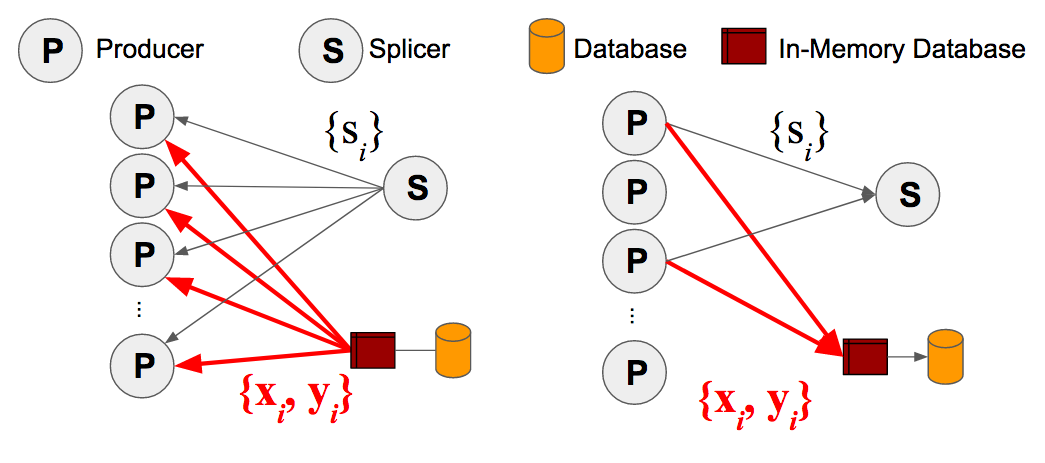
\includegraphics[width=19pc,angle=0]{figures/arch-parsplice.png}\\
%  \caption{ParSplice is a ready-heavy HPC application where producers use a
%  database for consistency. Replacing the single-node database with HXHIM
%  improves performance with load balancing.
%  \label{fig:arch-parsplice}}
%\end{figure}
%
%% Why is HXHIM a good fit?
%To show the efficacy of this approach, we examine the ParSplice molecular
%dynamics simulation application shown in Figure~\ref{fig:arch-parsplice}.
%ParSplice uses a single-node database for consistency, where producers, \(P\),
%push and pull coordinates, \{\(x_i, y_i\)\}, based on the segments,
%\{\(s_i\)\}, assigned by the splicer, \(S\). In this paper, we replace the
%database with a distributed key-value store designed for HPC enjoy performance
%optimizations for:
%
%\begin{itemize}
%  \item \texttt{put()} because of the distributed sync and load balancing based on:
%  \begin{itemize}
%    \item lazy synchronization with tombstones and RPCs
%    \item strong synchronization with consensus and blocking
%  \end{itemize}
%  \item \texttt{get()} because of the load balancing
%\end{itemize}
%
%It has 4 phases:
%
%\begin{enumerate}
%
%  \item splicer (S) tells producers (P) to compute segments for state \(s_i\)
%
%  \item P's pull initial coordinates \{\(x_i, y_i\)\} from database
%
%  \item a P inserts completed coordinates for segment \(s_i\) into database and
%  S broadcasts next segment(s) \(s_j\) 
%
%  \item P's pull new segment coordinates \{\(x_j, y_j\)\}
%\end{enumerate}
%
%, which has both a high computational footprint and data locality.
%The former suggests distribution to avoid hot spots while the latter encourages
%concentration to leverage the database's secondary indeices, bulk operations,
%and key redistribution functionality. 
%
%% Why is HXHIM a good fit?
%To show this approach at scale we study
%ParSplice~\cite{perez:jctc20150parsplice}, an HPC dynamics simulator that has
%both a high computation footprint, which suggests distribution to avoid hot
%spots, and data locality, which alternatively encourages concentration so the
%key-value store can use its functionality for secondary indices, bulk
%operations, and key redistribution. ParSplice uses both molecular dynamic (MD)
%and accelerated molecular dynamic methods (AMD) for simulations with long
%periods of inactivity and short periods of ``interesting" events.  Molecules in
%periods with many events are simulated with MD methods, which are exact but can
%only be run for a fixed, short period of time because the cumulative error
%grows so large. Alternatively, longer trajectories are simulated with AMD
%methods, which use statistics and parallelization to show the less precise
%state-to-tate trajectories. ParSplice tackles ``low-barrier problems", where
%the types of energy barriers separating states of the system are non-uniform
%(i.e. some require less energy than others). It chops long trajectories into
%parallelizable units called segments, where the segments can also be spliced
%together to form longer trajectories; this approach allows ParSplice to trade
%off accuracy for speed in a configurable way.
%
%% How is ParSplice implemented?
%ParSplice stores segments in a database while it runs. The splicer pastes
%segments generated by \(n\) producers.
%
%% What do we contribute?
%In this paper, we make the following contributions:
%
%\begin{enumerate}
%
%  \item protype that controls concentration and distribution using the bulk
%  operations, secondary indicies, and cursor types mechanisms
%  from~\cite{greenberg:hotstorage2015-mdhim}. 
%
%  \item quantifies benefits of server/client-side caching, many small messages,
%  and bulk operations.
%
%\end{enumerate}

\section{Background}

\subsection{ParSplice}
\label{sec:parsplice}

\begin{figure}[t]
  \noindent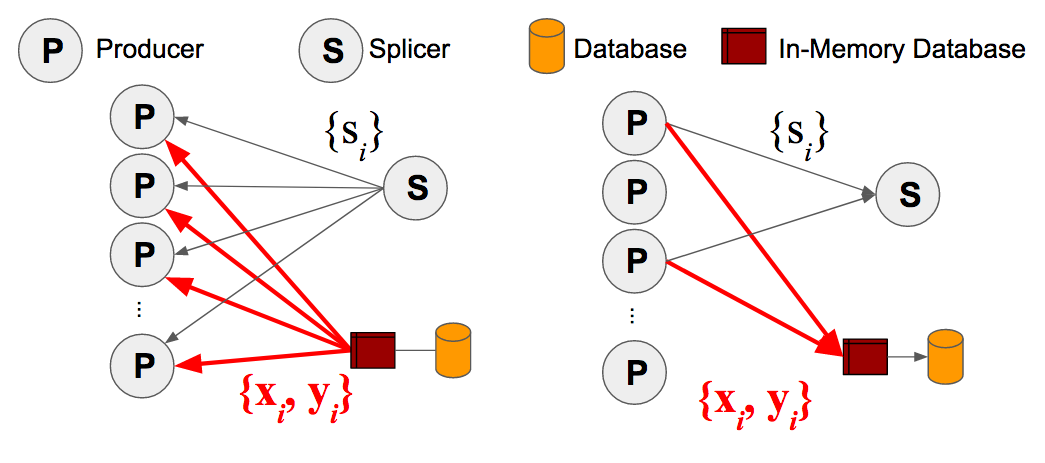
\includegraphics[width=19pc,angle=0]{figures/arch-parsplice.png}\\
  \caption{ParSplice is a ready-heavy HPC application where producers use a
  database for consistency. Replacing the single-node database with HXHIM
  improves performance with load balancing.
  \label{fig:arch-parsplice}}
\end{figure}


ParSplice~\cite{perez:jctc20150parsplice} is a molecular dynamics simulation
developed at LANL. It has 4 phases, as depicted in Figure~\ref{fig:arch-parsplice}:

\begin{enumerate}

  \item splicer (S) tells producers (P) to compute segments for state \(s_i\)

  \item P`s pull initial coordinates \{\(x_i, y_i\)\} from database

  \item a P inserts completed coordinates for segment \(s_i\) into database and
  S broadcasts next segment(s) \(s_j\) 

  \item P`s pull new segment coordinates \{\(x_j, y_j\)\}

\end{enumerate}

The database is single node (LevelDB or BerkeleyDB) with caches in front. Our
goal is to replace this architecture with a distributed key-value store to
solve the immediate sync problems that the ParSplice team is facting. Sliding
in something like MDHIM~\cite{greenberg:hotstorage2015-mdhim} has the added
benefit of enabling load balancing. ParSplice has distinct workload phases and
a well-known keyspace (Figure~\ref{fig:methodology-keyspace}) so its
performance should improve with better load balancing.

\subsection{MDHIM: Key-Value Store for HPC}
\label{sec:hxhim}

\begin{figure}[tb]
  \noindent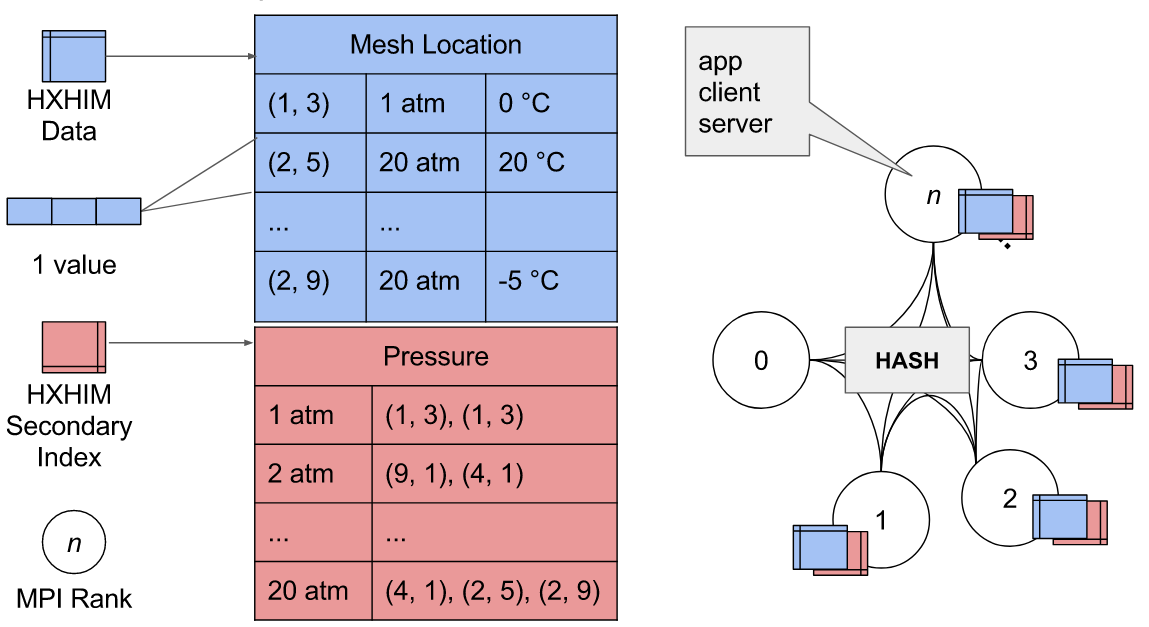
\includegraphics[width=19pc,angle=0]{figures/arch-hxhim.png}\\
  \caption{The MDHIM architecture.}
  \label{fig:arch-hxhim}
\end{figure}

% What is MDHIM
MDHIM is a key-value store designed for HPC architectures and multi-dimensional
data. It is based off MDHIM~\cite{greenberg:hotstorage2015-mdhim}, the
multi-dimensional indexing middleware. Figure~\ref{fig:arch-hxhim} has a crude
sketch of the MDHIM architecture. Each MPI rank has an instance of the
application, which has the client library linked in. An MPI rank can also have
a ``range server", which stores the key-value pairs in a local databse (either
LevelDB or MySQL). Data is located with a consistent hash, which is
configurable.

% What are the indexes?
The primary and secondary indices shown on the right side of
Figure~\ref{fig:arch-hxhim} are views of the data that the range server
manages.  The primary index is the same hash used by the global partitioner.
The secondary index or indices are user-defined tables organized in a different
way from the primary index. The goal of the secondary indices is to speed up
queries that need to aggregate dat ({\it e.g.} find the maximum values). In the
example, the range server and the key in the primary index is located with a
hash of the mesh location. The secondary index is organized by pressure, so
queries asking for a certain atmosphere can be serviced in O\(1\), consisting
of one lookup in the pressure index and one lookup into the primary index.

% Why is it tailored to HPC?
MDHIM tailors its mechanisms and policies to HPC, showing improved performance
over cloud-based key-value stores like Cassandra. It has cursor types for
walking the key-value store, bulk operations for exploiting data locality,
per-job server spawning, and pluggable backends for its local database and
network type (infiniband/RDMA). Its policies are flexible, supporting
customized partitioning strategies and user-defined secondary indices. This
allows the system to choose whether to send load to the client or server.

%\subsection{Comparing Mantle and MDHIM}
%\begin{table*}
%\centering
%\begin{tabular}[tb]{ r | l | l | l | l }
%                       & 
%                       & \multicolumn{1}{c|}{\centering Both} 
%                       & \multicolumn{1}{c|}{\centering Mantle/CephFS}
%                       & \multicolumn{1}{c}{\centering MDHIM}
%                       \\\hline
%  workload   & characteristics     & small/frequent requests  & data access            & data management \\
%             & write-intensive     & partition across cluster & fragment directories*  & NOT IMPLEMENTED \\
%             & read-intensive      & replicate across cluster & copy directories*      & NOT IMPLEMENTED \\\hdashline
%  system     & measure workload    & yes                      & directory temperature  & range server counts \\
%  mechanisms & measure utilization & yes                      & CPU, network, memory   & range server buffer size \\
%             & migrate resources   & almost                   & \texttt{export\_dir()} & \texttt{mdhimB}\{\texttt{Get}, \texttt{Put}\}\texttt{()} \\
%             & partition resources & yes                      & subtrees \& dirfrags   & secondary index, cursor type, bulk operations\\\hdashline
%  migration  & interval            & configurable             & every 10 seconds       & every query \\
%  decisions  & global state        & decentralized decisions  & heartbeats for metrics & NOT IMPLEMENTED \\
%  \multicolumn{5}{c}{}\\
%  \multicolumn{5}{c}{\tiny *Mechanisms implemented in CephFS, not integrated into Mantle}
%\end{tabular}
%\caption{Comparing the design goals and implementatons of Mantle and MDHIM.}
%\label{fig:arch-comparison}
%\end{table*}
%
%% Why are the designed for the same type of workload?
%The ``Both" column of Table~\ref{fig:arch-comparison} shows how Mantle and
%MDHIM have similar designs. The workloads are very similar as the the services
%respond to small and frequent requests, which results in hot spots and flash
%crowds. As a result, popularity of the data, not the size, drives distribution
%in both systems. Both workloads also have data locality so the systems have
%mechanisms for leveraging requests with similar semantic meaning.  Finally, the
%overall design of both systems is decentralized meaning that there is no
%centralized scheduler and each server has an inconsistent global view.
%
%% What are the challenges?
%Despite the similarities, integrating the Mantle API with MDHIM has both design
%and technical challenges. Mantle is reactive to the workload as opposed to
%MDHIM migrations, which are triggered based on the request type. As a result,
%Mantle has functionality for exchanging server utilization (CPU, network,
%memory) and workload (tracks request types). MDHIM 
%
%
%%This paper takes the API and load balancers designed in
%%Mantle~\cite{sevilla:sc15-mantle}, the programmabile file system metadata load
%%balancer for Ceph, and applies them to
%%MDHIM~\cite{greenberg:hotstorage2015-mdhim}, the distributed key-value store
%%designed for HPC.
%
%
%
%Results should show, In order from most likely to least likely:
%
%\begin{enumerate}
%
%  \item HPC key-value store workloads are structured (because they are mostly
%  workflows and simulations) that their job phases can be learned and exploited
%  using dynamic load balancing policies.
%
%  \item HPC key-value store workloads are so structured that one
%  policy-fits-all
%
%  \item HPC key-value store workloads are not structured enough to be learned
%
%  \item HPC key-value store workload hotspots/flash crowds are too fast to be
%  exploited
%
%\end{enumerate}

\section{Methodology: Extracting Mantle Library}

\begin{itemize}
  \item C bindings for Mantle
\end{itemize}

\subsection{Pluggable Interfaces}

\begin{figure}[tb]
  \noindent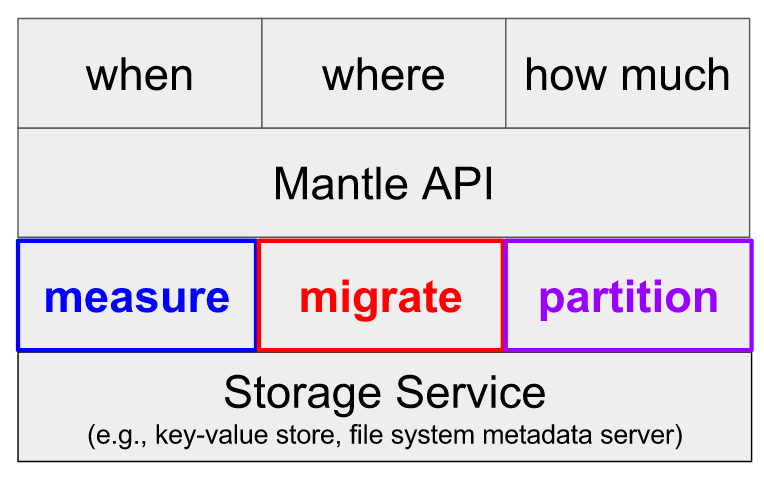
\includegraphics[width=19pc,angle=0]{figures/mantle-pluggable-interfaces.png}\\
  \caption{The storage service must: \textcolor{blue}{\textbf{measure}}
  resource usage, \textcolor{red}{\textbf{migrate}} resources, and
  \textcolor{purple}{\textbf{partition}} resources. }
  \label{fig:mantle-pluggable-interfaces}
\end{figure}

\subsubsection{Measure}

The metrics measured should help the system decide ``when" to migrate server
load. They should:

\begin{itemize}
  \item tell us about the state of the server or cluster
  \item provide some value of load, so we can partition/send it
\end{itemize}

In Ceph: global and local metrics ({\it e.g.}, CPU utilization, file system operation counts) \\

In HXHIM: ???\\

\subsubsection{Migrate}

In Ceph: \texttt{export\_dir()}

In HXHIM: \texttt{mdhimBPut()}, \texttt{mdhimBGet()}, ``adjusting ... keys" ???

\subsubsection{Partition}

In Ceph: subtrees and directory fragments

In HXHIM: secondary indices, cursor types, bul operations

\section{Conclusion}

\begin{enumerate}
  \item analysis of Parsplice keyspace
  \item using a modern distributed kv store
  \item positive effects of Mantle
\end{enumerate}


%% In all cases, if there is only one entry of this type within
%% the higher level heading, use the star form: 
%%
%\section{Section title}
%\subsection*{subsection}
%
%text... and some citations \cite{Kuji_Nakajima2002}
%
%\section{Section title}

%vs

% \section{Section title}
% \subsection{subsection one}
% text...
% \subsection{subsection two}
% \section{Section title}

%%%
% \section{First primary heading}

% \subsection{First secondary heading}

% \subsubsection{First tertiary heading}

% \paragraph{First quaternary heading}

%%%%%%%%%%%%%%%%%%%%%%%%%%%%%%%%%%%%%%%%%%%%%%%%%%%%%%%%%%%%%%%%%%%%%
% ACKNOWLEDGMENTS
%%%%%%%%%%%%%%%%%%%%%%%%%%%%%%%%%%%%%%%%%%%%%%%%%%%%%%%%%%%%%%%%%%%%%
%
\acknowledgments
Start acknowledgments here.

%%%%%%%%%%%%%%%%%%%%%%%%%%%%%%%%%%%%%%%%%%%%%%%%%%%%%%%%%%%%%%%%%%%%%
% APPENDIXES
%%%%%%%%%%%%%%%%%%%%%%%%%%%%%%%%%%%%%%%%%%%%%%%%%%%%%%%%%%%%%%%%%%%%%
%
% Use \appendix if there is only one appendix.
%\appendix

% Use \appendix[A], \appendix}[B], if you have multiple appendixes.
%\appendix[A]

%% Appendix title is necessary! For appendix title:
%\appendixtitle{}

%%% Appendix section numbering (note, skip \section and begin with \subsection)
% \subsection{First primary heading}

% \subsubsection{First secondary heading}

% \paragraph{First tertiary heading}

%% Important!
%\appendcaption{<appendix letter and number>}{<caption>} 
%must be used for figures and tables in appendixes, e.g.,
%
%\begin{figure}
%\noindent\includegraphics[width=19pc,angle=0]{figure01.pdf}\\
%\appendcaption{A1}{Caption here.}
%\end{figure}
%
% All appendix figures/tables should be placed in order AFTER the main figures/tables, i.e., tables, appendix tables, figures, appendix figures.
%
%%%%%%%%%%%%%%%%%%%%%%%%%%%%%%%%%%%%%%%%%%%%%%%%%%%%%%%%%%%%%%%%%%%%%
% REFERENCES
%%%%%%%%%%%%%%%%%%%%%%%%%%%%%%%%%%%%%%%%%%%%%%%%%%%%%%%%%%%%%%%%%%%%%
% Make your BibTeX bibliography by using these commands:
\bibliographystyle{abbrv}
\bibliography{references}


%%%%%%%%%%%%%%%%%%%%%%%%%%%%%%%%%%%%%%%%%%%%%%%%%%%%%%%%%%%%%%%%%%%%%%
%% TABLES
%%%%%%%%%%%%%%%%%%%%%%%%%%%%%%%%%%%%%%%%%%%%%%%%%%%%%%%%%%%%%%%%%%%%%%
%%% Enter tables at the end of the document, before figures.
%%%
%%
%\begin{table}[t]
%\caption{This is a sample table caption and table layout.  Enter as many tables as
%  necessary at the end of your manuscript. Table from Lorenz (1963).}\label{t1}
%\begin{center}
%\begin{tabular}{ccccrrcrc}
%\hline\hline
%$N$ & $X$ & $Y$ & $Z$\\
%\hline
% 0000 & 0000 & 0010 & 0000 \\
% 0005 & 0004 & 0012 & 0000 \\
% 0010 & 0009 & 0020 & 0000 \\
% 0015 & 0016 & 0036 & 0002 \\
% 0020 & 0030 & 0066 & 0007 \\
% 0025 & 0054 & 0115 & 0024 \\
%\hline
%\end{tabular}
%\end{center}
%\end{table}
%
%%%%%%%%%%%%%%%%%%%%%%%%%%%%%%%%%%%%%%%%%%%%%%%%%%%%%%%%%%%%%%%%%%%%%%
%% FIGURES
%%%%%%%%%%%%%%%%%%%%%%%%%%%%%%%%%%%%%%%%%%%%%%%%%%%%%%%%%%%%%%%%%%%%%%
%%% Enter figures at the end of the document, after tables.
%%%
%%
%\begin{figure}[t]
%  \noindent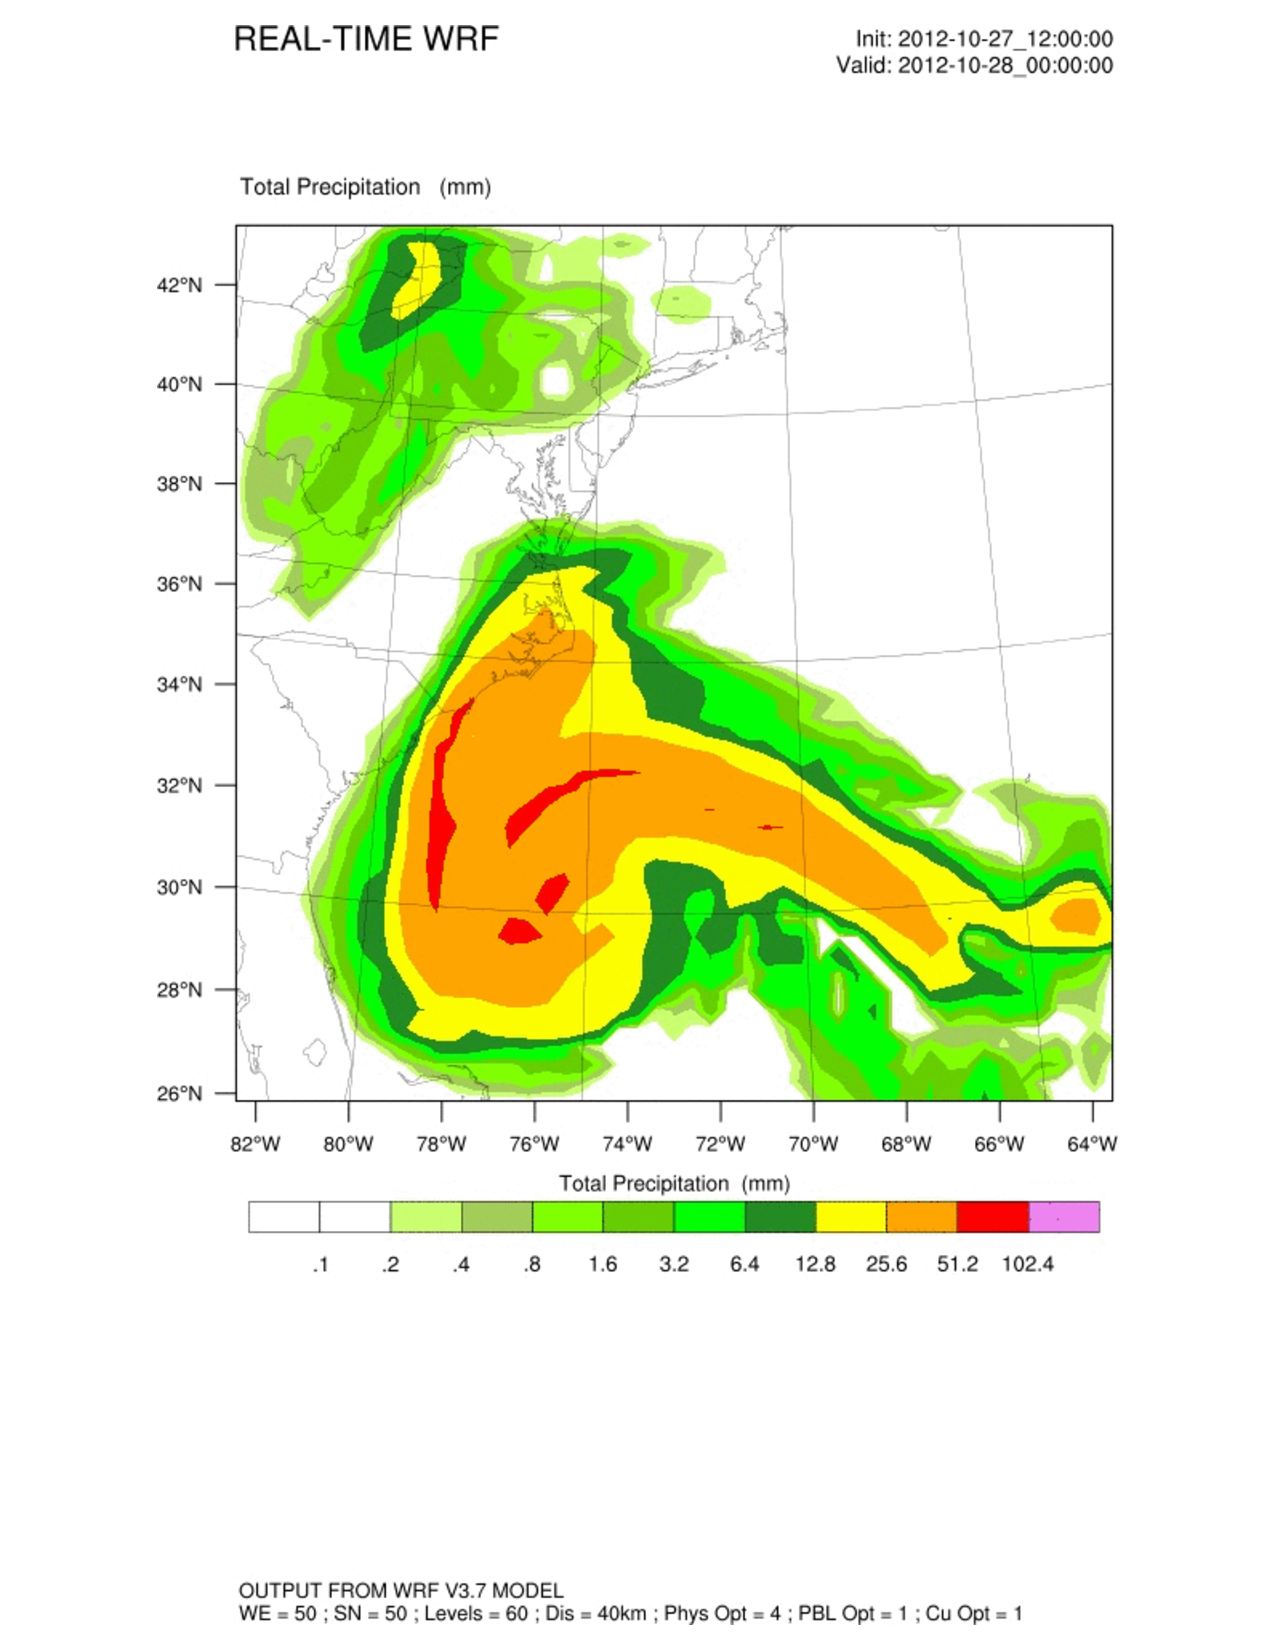
\includegraphics[width=19pc,angle=0]{figures/Fig02.pdf}\\
%  \caption{Enter the caption for your figure here.  Repeat as
%  necessary for each of your figures.}\label{f1}
%\end{figure}

\end{document}
